\subsubsection{Группа}
    Рассмотрим некоторую группу $G$, его фактор-группу $G/G'$ по коммутанту 
    $G'$ и следующую диаграмму

    \begin{figure}[h]
        \centering
        \[\xymatrix{
            G \ar[rr]^{\textstyle{\tau}} \ar[rrdd]_{\textstyle{\chi}} & & G/G'\ar[dd]^{\textstyle{\chi_{ab}}} \\
            & & \\
            & & \mathbb{C}
        }\]
        \caption{}
        \label{cd_ab}
    \end{figure}

    Здесь $\tau: g \mapsto gG'$ --- канонический гомоморфизм; $\chi$, 
    $\chi_{ab}$ --- характеры групп $G$ и $G/G'$ соответственно.

    Оказывается, что 
    \begin{statement} для любого $\chi : G \to \mathbb{C}$ существует и при том 
        единственный характер $\chi_{ab} : G/G' \to \mathbb{C}$ такой, что диаграмма 
        \eqref{cd_ab} коммутативна, т.е. 
        \[\chi = \chi_{ab} \circ \tau.\]
    \end{statement}

    \begin{proof} Действительно, потребуем для любого $g \in G$
    \[\chi(g) = \chi_{ab} \circ \tau (g),\]
    тогда
    \[\chi(g) = \chi_{ab} (gG'),\]
    и $\chi_{ab}$ задан на $G/G'$ однозначно.

    Более того $\chi_{ab}$ задан корректно, т.к. для $\forall f \in gG'$ 
    $\exists h \in G': f = gh$, но по определению коммутанта существуют такие 
    $a$ и $b$, что $h = aba^{-1}b^{-1}$, откуда $f = gaba^{-1}b^{-1}$, и 
    \[\chi(f) = \chi(gaba^{-1}b^{-1}) 
    = \chi(g) + \chi(a) + \chi(b) - \chi(a) - \chi(b) = \chi(g),\]
    то есть,
    \begin{equation}\label{eq_chi_factor}
        \chi(f) = \chi(g),\text{ для любых $f$ и $g$ из одного смежного по $G'$ класса.}
    \end{equation}
    
    Очевидно, что $\chi_{ab}$ --- характер:
    \[\chi_{ab}(gf G') = \chi(gf) = \chi(g) + \chi(f) = \chi_{ab}(gG') + \chi_{ab}(fG').\]
    \end{proof}
    
    \begin{remark} Попутно доказано важное для понимания происходящего 
        утверждение \eqref{eq_chi_factor}, показывающее, что факторизация 
        группы по коммутанту $G'$ разбивает ее также и на "<области постоянства"> 
        характера (рис. \ref{img_chi_factor}). Становится яcно, что вместо 
        рассмотрения характера $\chi$ на всей группе, достаточно пронаблюдать 
        лишь за его "<действием с точностью до $G'$">, т.е. за определяемым им 
        на $G/G'$ характере $\chi_{ab}$.
    \end{remark}
    
    \begin{figure}[th]
        \centering
        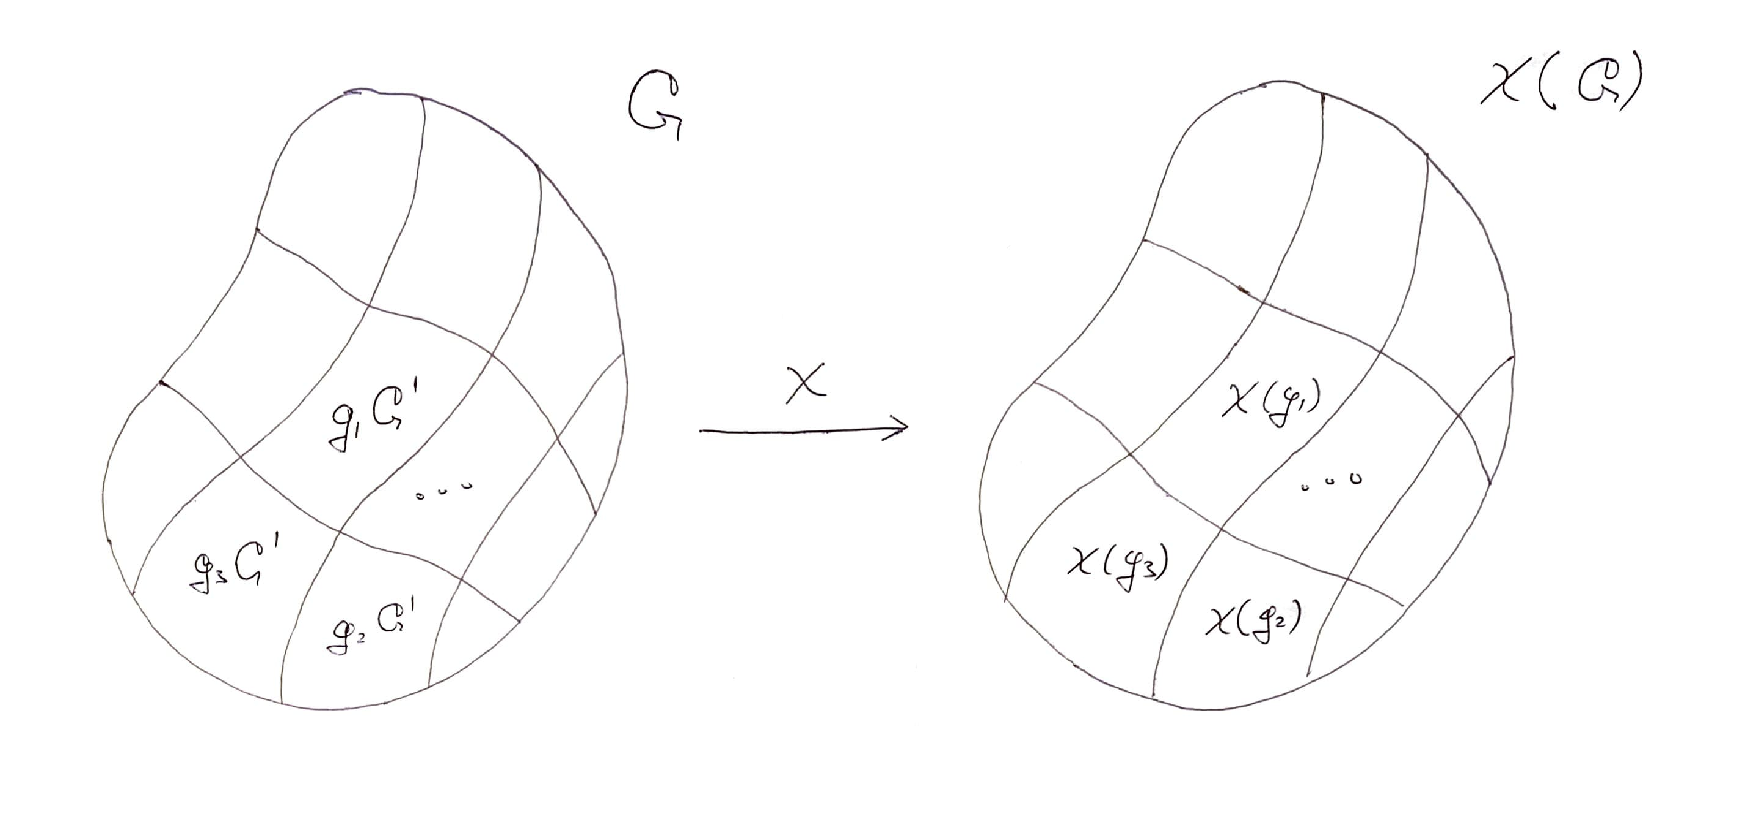
\includegraphics[width=\textwidth]{pictures/chips}
        \caption{}
        \label{img_chi_factor}
    \end{figure}

    Обратно,
    \begin{statement} характер $\chi_{ab}$ однозначно задает $\chi$, как 
        \[\chi = \chi_{ab}\circ \tau\]
    \end{statement}
    Утверждение представляется очевидным.

    Так, построено взаимооднозначное отображение $t: \chi_{ab} \mapsto 
    \chi_{ab} \circ \tau = \chi$ между характерами группы и ее абелизации 
    (т.е. фактор группы по коммутанту). Покажем, что отображение $t$ является 
    гомоморфизмом (а следовательно и изоморфизмом) линейных пространств.

    Действительно, для любого $g \in G$
        \begin{multline*}
        t(c_1\chi_{ab}^1 + c_2\chi_{ab}^2)(g) 
        = (c_1\chi_{ab}^1 + c_2\chi_{ab}^2) \circ \tau (g) = \\
        = (c_1\chi_{ab}^1 + c_2\chi_{ab}^2) (gG')
        = c_1\chi_{ab}^1 (gG') + c_2\chi_{ab}^2 (gG') = \\
        = c_1\chi_{ab}^1 \circ \tau (g) + c_2\chi_{ab}^2 \circ \tau (g)
        = c_1 t(\chi_{ab}^1)(g) + c_2 t(\chi_{ab}^2)(g).
        \end{multline*}
    Тем самым доказано следующее
    \begin{statement}
        Пространства характеров группы $G$ и ее абелизации $G/G'$ изоморфны. 
        Конкретно, изоморфизм имеет вид:
        \begin{equation}\label{iso_GG'}
            t: G/G' \to G.\quad t: \chi_{ab} \mapsto \chi_{ab} \circ \tau,
        \end{equation}
        где $\tau$ --- канонический гомоморфизм $G \to G/G'$.
    \end{statement}
    
    Последнее утверждение позволяет нам свести задачу изучения характеров
    группы $G$ к рассмотрению характеров на $G/G'$ --- группе, абелевой по 
    определению.